\documentclass{report}

\usepackage{amsmath}

\usepackage{graphicx} 

\usepackage[hidelinks]{hyperref}
\usepackage{amsmath}

\usepackage{float}

\DeclareMathOperator{\sinc}{sinc}
\DeclareMathOperator{\rect}{rect}


\usepackage[square,sort,comma,numbers]{natbib}
\usepackage[colorinlistoftodos]{todonotes}
\usepackage{listings}
\definecolor{darkgreen}{rgb}{0.0, 0.4, 0.0}
\lstset{
language=Matlab,
basicstyle=\color{black},
commentstyle=\color{green!60!black},
stringstyle=\color{purple},
showstringspaces=false,
keywordstyle=\color{blue},
emph=[1]{for,end,break},
emphstyle=[1]\color{red},
numbers=left,
numberstyle={\tiny \color{black}},
numbersep=12pt}
\usepackage{multicol}




\font\fontTitle=cmr12 at 30pt
\setlength{\parskip}{\baselineskip}%

\title{\fontTitle Signal Processing Project  }
\author{
  \Large Niranjan Gopal \\
  \normalsize IMT2022543 \\
  \normalsize \texttt{niranjan.gopal@iiitb.ac.in}
    \\ \\ \\ \\
  \Large Chirag M V\\
  \normalsize IMT2022583 \\
  \normalsize \texttt{MV.Chirag@iiitb.ac.in}
    \\ \\ \\ \\
  \Large Vaibhav Bajoriya \\
  \normalsize IMT2022574 \\
  \normalsize \texttt{Vaibhav.Bajoriya@iiitb.ac.in}
}
\date{ March 2024 }

\begin{document}

\maketitle



\tableofcontents

\chapter{Introduction }



\section{Generating and Transmitting any 5 signals}


% write briefly about the problem statement.

The transmission and reception of audio signals play a vital role in various applications, from telecommunications to multimedia systems. In this experiment, we aim to explore the process of generating, transmitting, and receiving audio signals using speakers and microphones. The primary objective is to understand the behavior of audio signals as they propagate through space and are captured by a receiving device.

To begin, we will generate five distinct audio signals using MATLAB , ensuring they adhere to the specifications of the microphone used for recording. These signals will include various types, such as sinusoidal, square, triangular waves, and possibly voice recordings or music excerpts. Each signal will be saved as a .wav file, along with specifying the sampling frequency required for playback.

Next, we will set up a transmission-reception system by placing a speaker and a microphone at different distances apart, ranging from 1 meters to 5 meters. This setup will enable us to analyze the effects of distance on the transmitted and received signals. By capturing the received signals using a microphone connected to another laptop, we can compare them with the original transmitted signals.

Furthermore, we will examine the time-domain and frequency-domain characteristics of both the transmitted and received signals. This analysis will provide insights into how signal propagation affects their temporal and spectral properties. By comparing these plots, we can assess any distortions or alterations incurred during transmission and reception.

     
\section{Profiles of Generated Signals }

\hspace{0.4cm}
{
\textbf{Signal 1:}
\[ y_1 = \cos(2\pi \times 5000 \times t) \]

\textbf{Signal 2:}
\[ y_2 = 0.9 \sin(2\pi \times 1000 \times t) \]

\textbf{Signal 3:}
\[ y_3 = 0.5 \sin(2\pi \times 3000 \times t) + 0.3 \cos(2\pi \times 6000 \times t) \]

\textbf{Signal 4:}
\[ y_4 = 0.8 \cdot \text{triangle}(2 \pi \times 2000 \times t, 0.5) \]

\textbf{Signal 5:}
\[ y_5 = 0.3 \cos(2\pi \times 5000 \times t) + \text{noise} \]
}



\subsection{Profiles of Generated Signals in Time Domain}
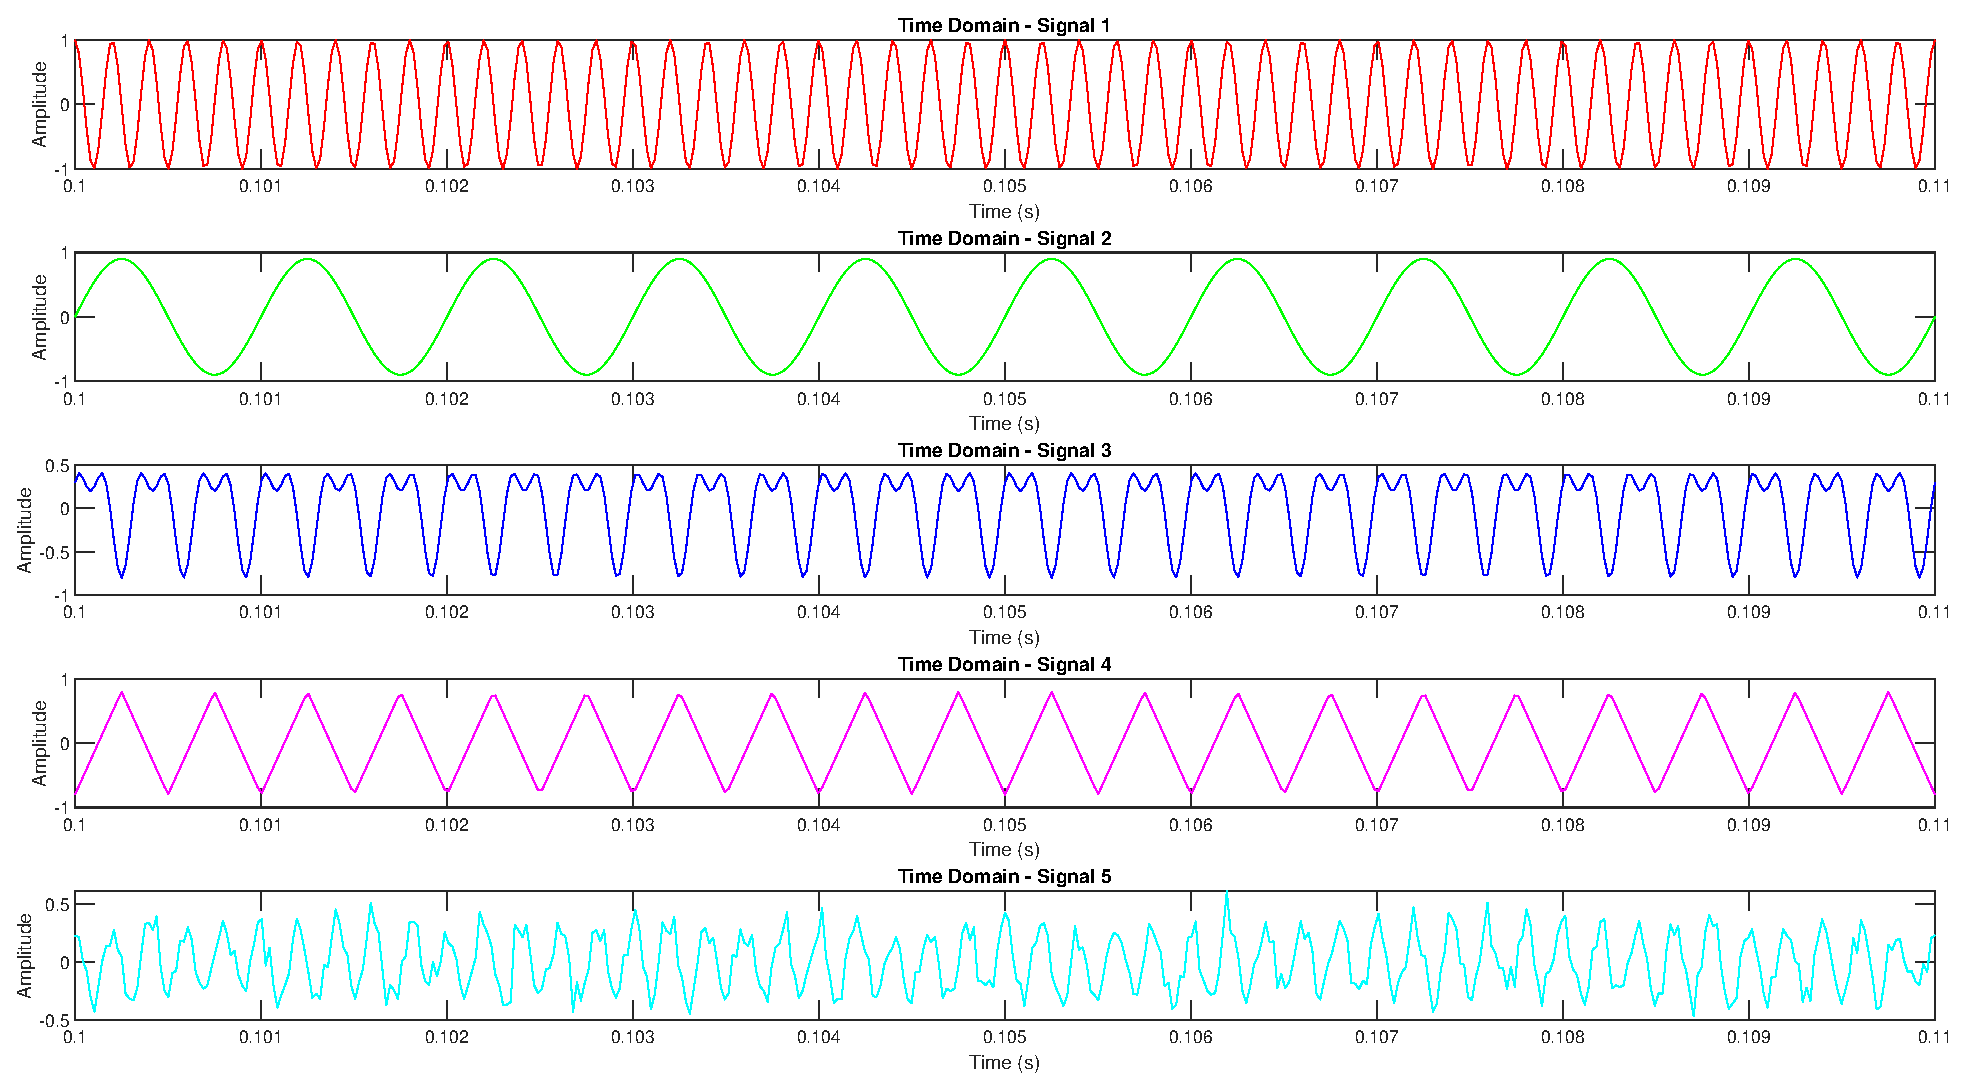
\includegraphics[width=1\linewidth]{Time_Domain_Signals.eps}


\subsection{Profiles of Generated Signals in Frequency Domain}
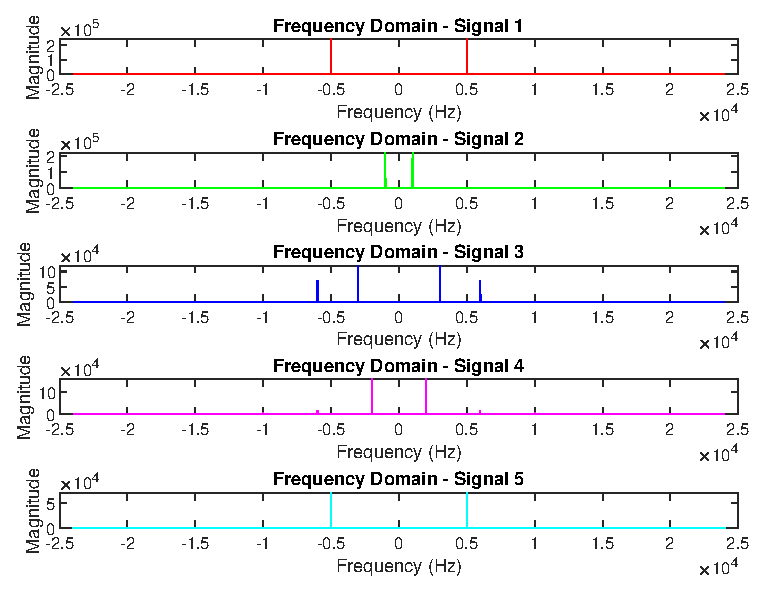
\includegraphics[width=1\linewidth]{Frequency_Domain_Signals.eps}


\section{Performing the Experiment}

We generated five different signals and saved as .wav files with a sampling frequency of 48 kHz. Using a microphone, we collected these signals at distances of 1m, 3m, and 5m from the speaker. Analyzing the frequency response revealed variations in signal amplitude and frequency content with distance. Comparing time-domain and frequency-domain plots showed distortions and attenuation during transmission. 

Reason for choosing distances 1m, 3m, 5m instead of 3m, 5m, 7m:
When we transmitted the signals at distances 3m, 5m, 7m, the analysis was valid for 3m and 5m, but at 7m, the presence of noise was sufficiently large to affect the receiver from clearly receiving the signal. So, it was decided that the signal would be received at 1m instead of 7m, so that the effect of noise reduces.
% Why we are doing 1,3,5 instead of 3,5,7 

These findings highlight the impact of distance on signal integrity and provide insights into speaker-microphone system performance.

\newpage
\subsection{Profiles of Received Signal at 1 m }


\subsubsection{Signal - 1}

$$ y_1 = \cos(2\pi \times 5000 \times t) $$
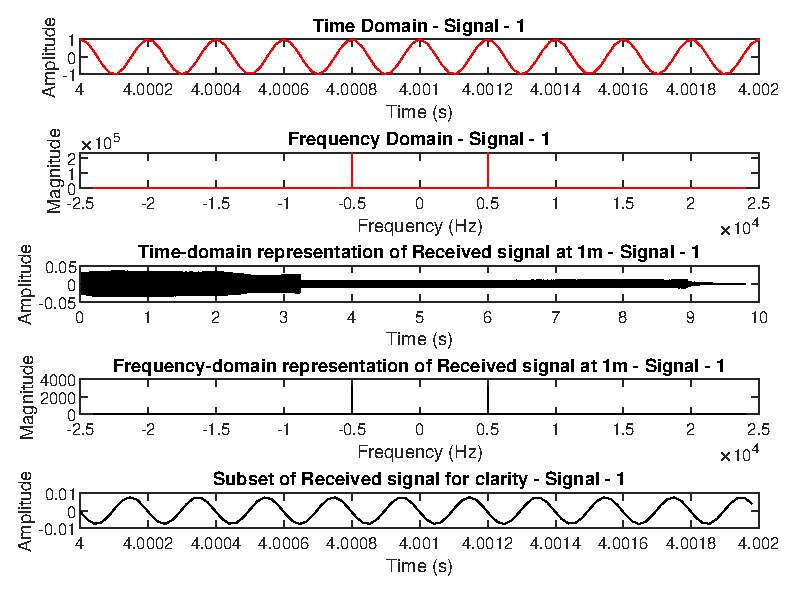
\includegraphics[width=1.1\linewidth]{1_1.eps}


\newpage
\subsubsection{Signal - 2}

$$ y_2 = 0.9 \sin(2\pi \times 1000 \times t) $$
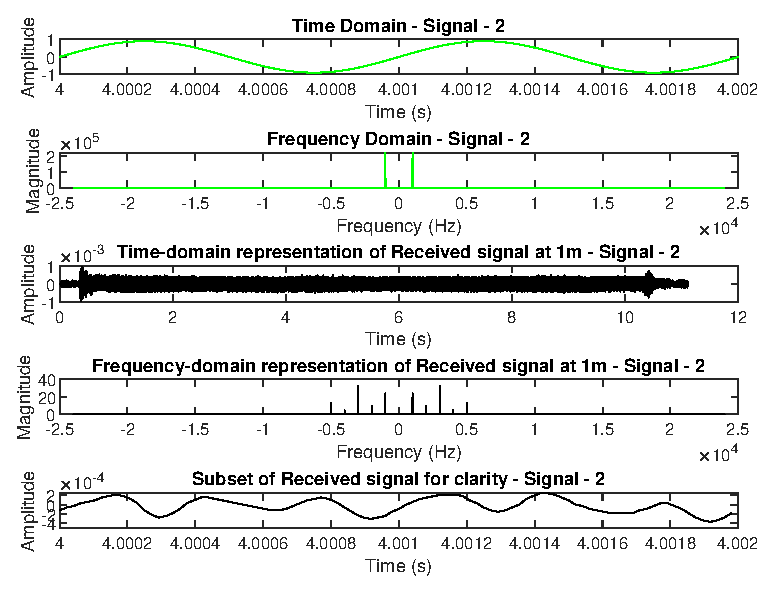
\includegraphics[width=1.1\linewidth]{1_2.eps}


\newpage
\subsubsection{Signal - 3}

$$ y_3 = 0.5 \sin(2\pi \times 3000 \times t) + 0.3 \cos(2\pi \times 6000 \times t) $$
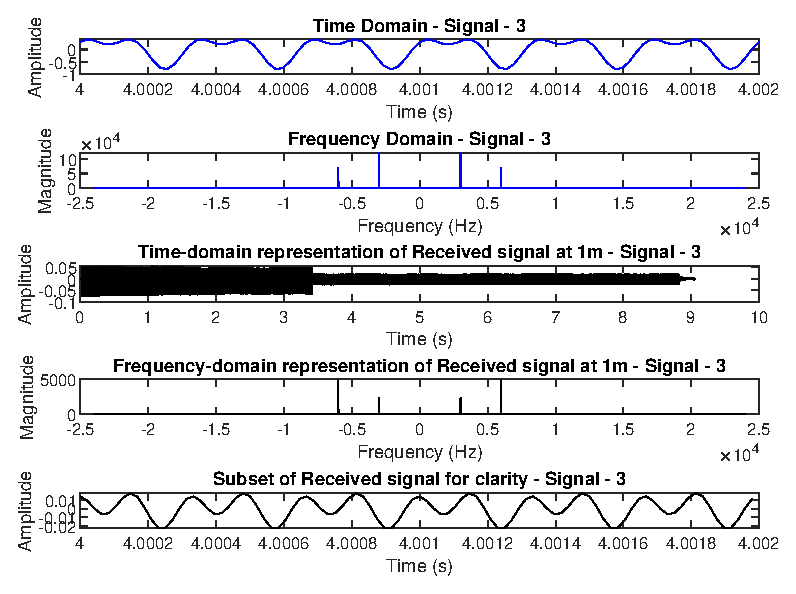
\includegraphics[width=1.1\linewidth]{1_3.eps}




\newpage
\subsubsection{Signal - 4}

$$ y_4 = 0.8 \cdot \text{triangle}(2 \pi \times 2000 \times t, 0.5) $$
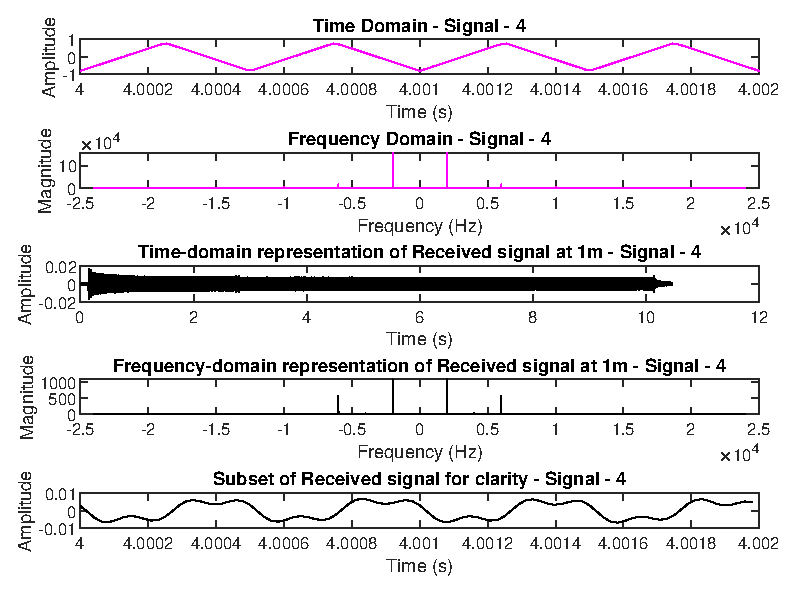
\includegraphics[width=1.1\linewidth]{1_4.eps}


\subsubsection{Important Inferences}

\begin{itemize}
    \item Recall that the frequency domain representation of a Triangular signal is  a $\sinc^2(f)$ function, which is band-unlimited. 
    \item The signal should have appeared as a smoother version of the transmitted triangle due to selective omission of higher frequencies. ( windowed version of $\sinc^2(f)$ )
    \item However, what we observe is a much more erratic signal, possibly arising not just from the selective omission of frequencies during windowing but also due to the effects of attenuation, distortion, and noise inherent in the transmission channel.
    \item This observation remains same for all distance of separations.
\end{itemize}






\newpage
\subsubsection{Signal - 5}

$$ y_5 = 0.3 \cos(2\pi \times 5000 \times t) + \text{noise} $$
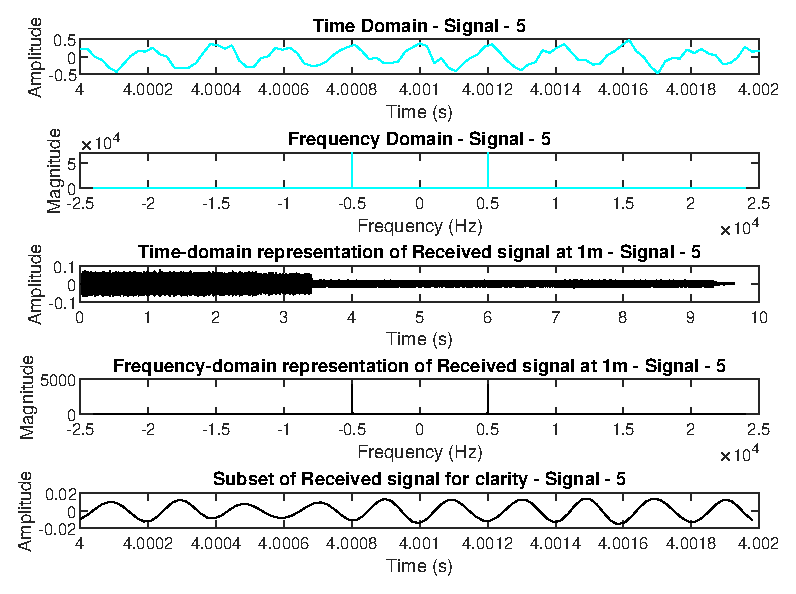
\includegraphics[width=1.1\linewidth]{1_5.eps}

\subsubsection{Important Inferences}
\begin{itemize}
\item Even though we sent a signal onto which we ourselves added noise, the received signal very much looks like the original signal without noise.
\item This is because of the noise cancelling capabilities of the microphone
\item This observation also remains same for all distance of separations.
\end{itemize}


\newpage
\subsection{Profiles of Received Signal at 3 m }


\subsubsection{Signal - 1}

$$ y_1 = \cos(2\pi \times 5000 \times t) $$
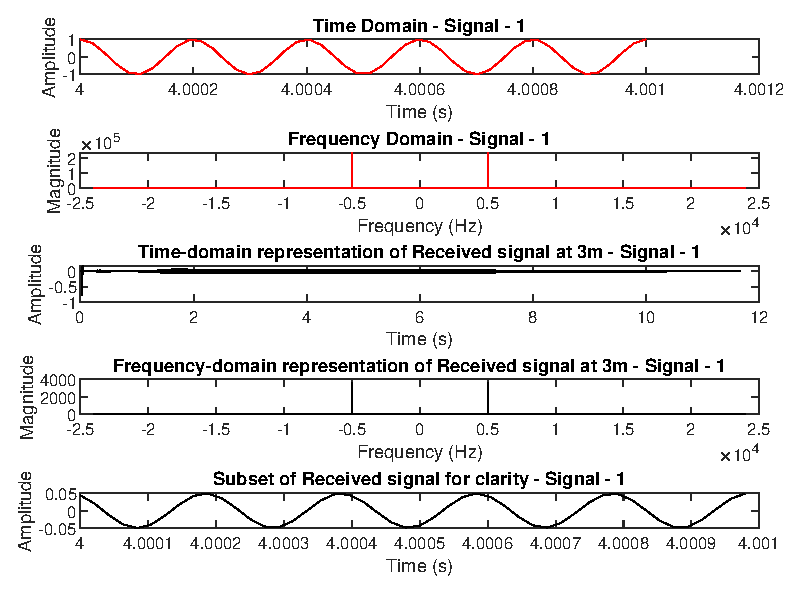
\includegraphics[width=1.1\linewidth]{3_1.eps}

\newpage
\subsubsection{Signal - 2}

$$ y_2 = 0.9 \sin(2\pi \times 1000 \times t) $$

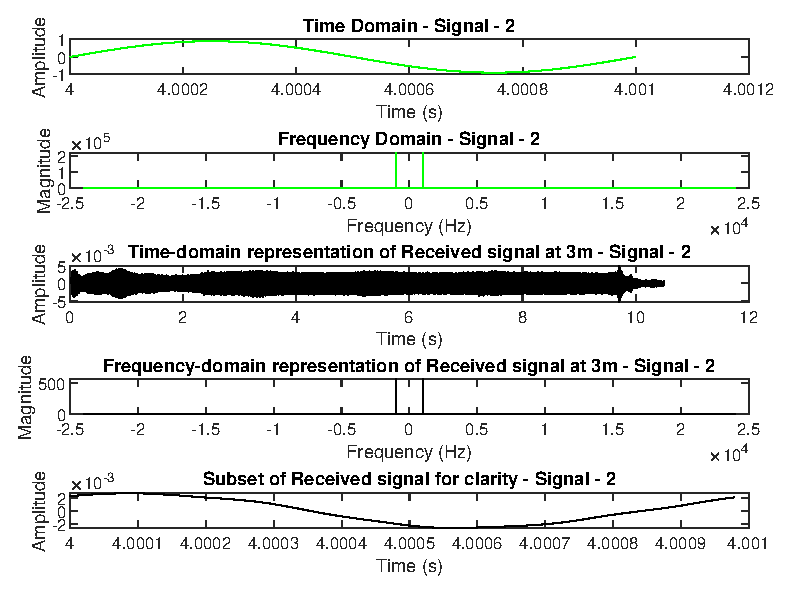
\includegraphics[width=1.1\linewidth]{3_2.eps}


\newpage
\subsubsection{Signal - 3}

$$ y_3 = 0.5 \sin(2\pi \times 3000 \times t) + 0.3 \cos(2\pi \times 6000 \times t) $$
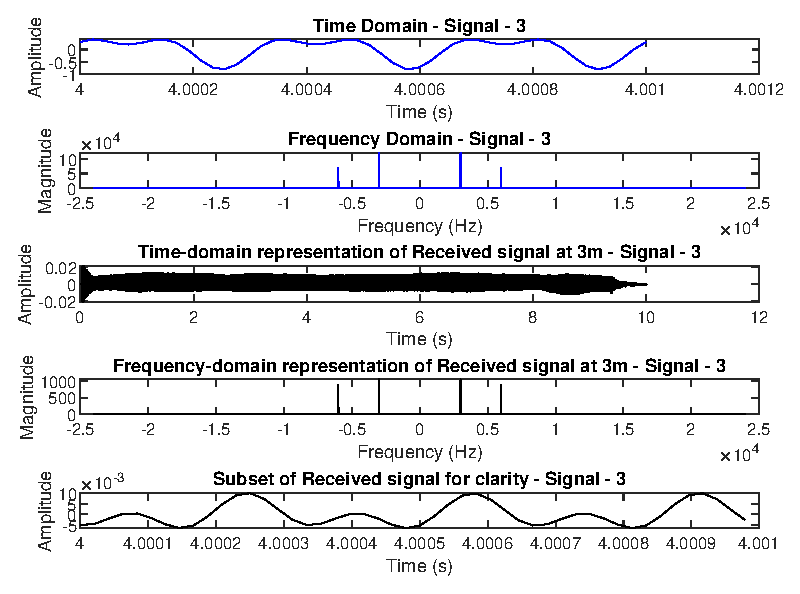
\includegraphics[width=1.1\linewidth]{3_3.eps}


\newpage
\subsubsection{Signal - 4}

$$ y_4 = 0.8 \cdot \text{triangle}(2 \pi \times 2000 \times t, 0.5) $$
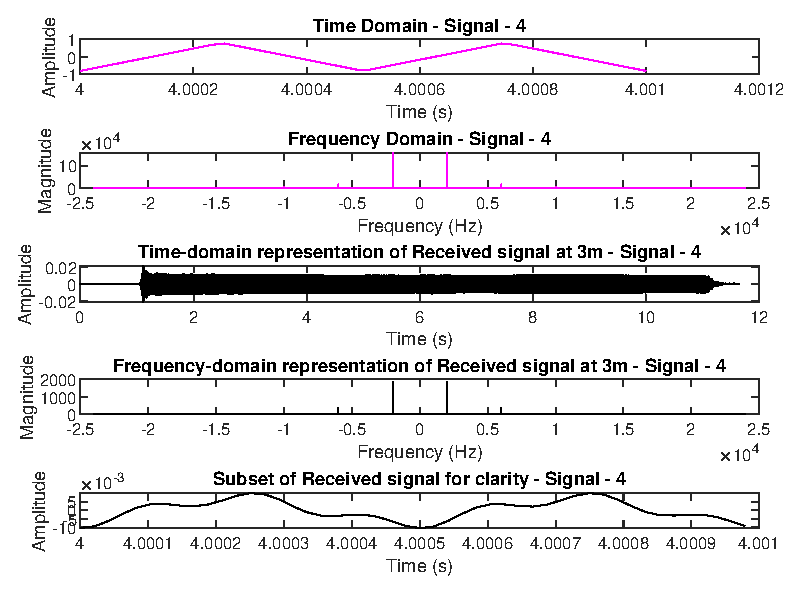
\includegraphics[width=1.1\linewidth]{3_4.eps}


\newpage
\subsubsection{Signal - 5}

$$ y_5 = 0.3 \cos(2\pi \times 5000 \times t) + \text{noise} $$
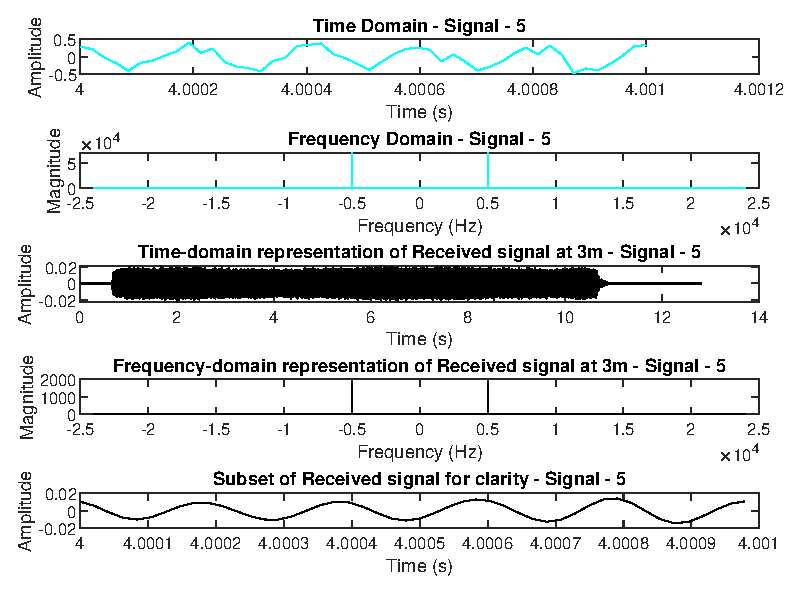
\includegraphics[width=1.1\linewidth]{3_5.eps}


\newpage
\subsection{Profiles of Received Signal at 5 m }


\subsubsection{Signal - 1}

$$ y_1 = \cos(2\pi \times 5000 \times t) $$
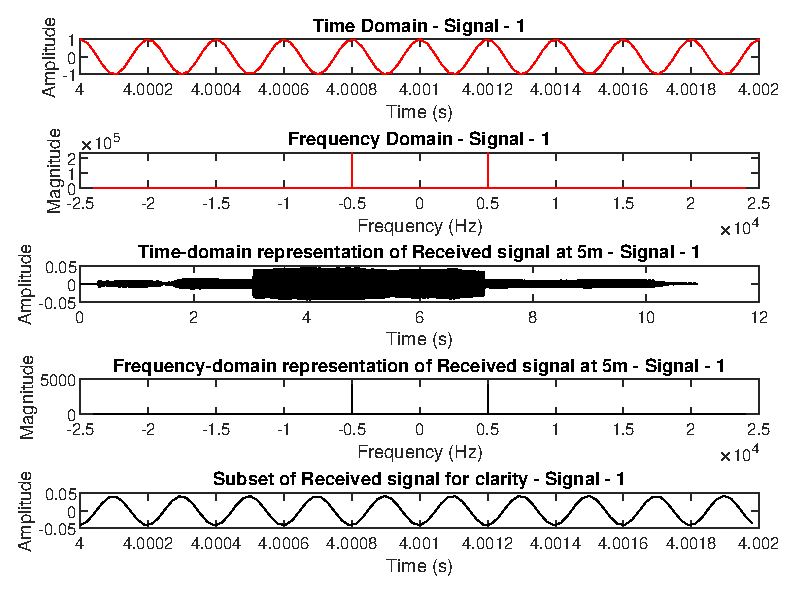
\includegraphics[width=1.1\linewidth]{5_1.eps}

\newpage
\subsubsection{Signal - 2}

$$ y_2 = 0.9 \sin(2\pi \times 1000 \times t) $$
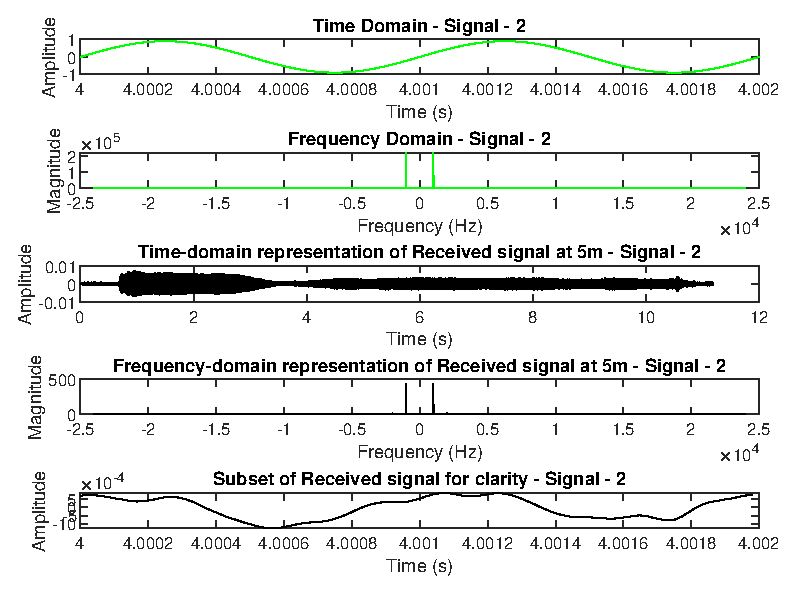
\includegraphics[width=1.1\linewidth]{5_2.eps}


\newpage
\subsubsection{Signal - 3}

$$ y_3 = 0.5 \sin(2\pi \times 3000 \times t) + 0.3 \cos(2\pi \times 6000 \times t) $$
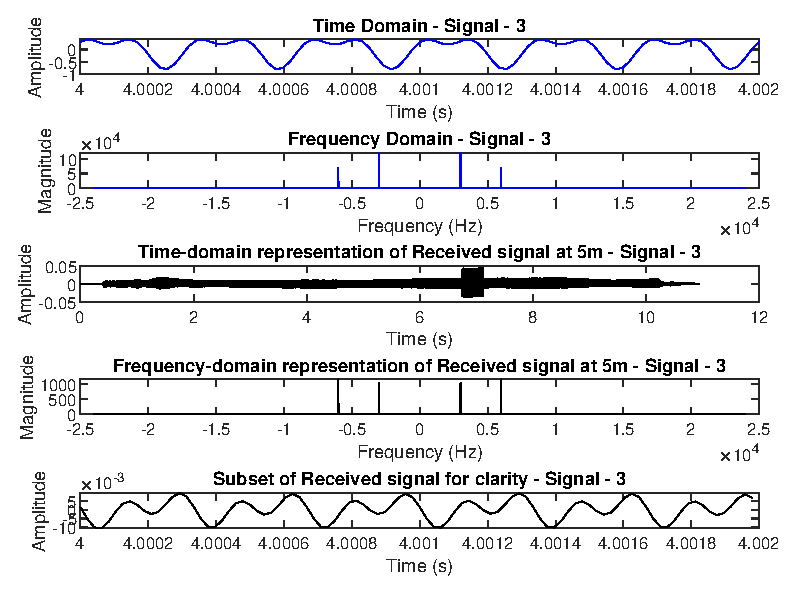
\includegraphics[width=1.1\linewidth]{5_3.eps}


\newpage
\subsubsection{Signal - 4}

$$ y_4 = 0.8 \cdot \text{triangle}(2 \pi \times 2000 \times t, 0.5) $$
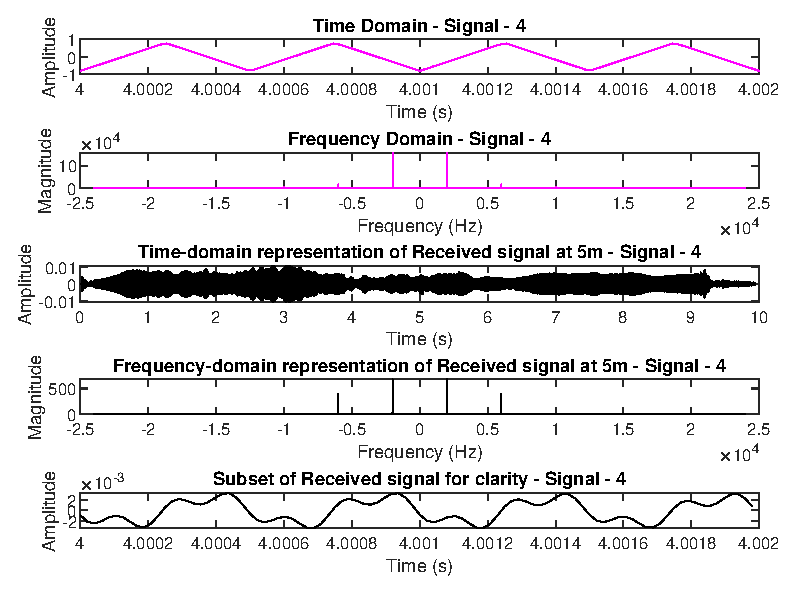
\includegraphics[width=1.1\linewidth]{5_4.eps}


\newpage
\subsubsection{Signal - 5}

$$ y_5 = 0.3 \cos(2\pi \times 5000 \times t) + \text{noise} $$
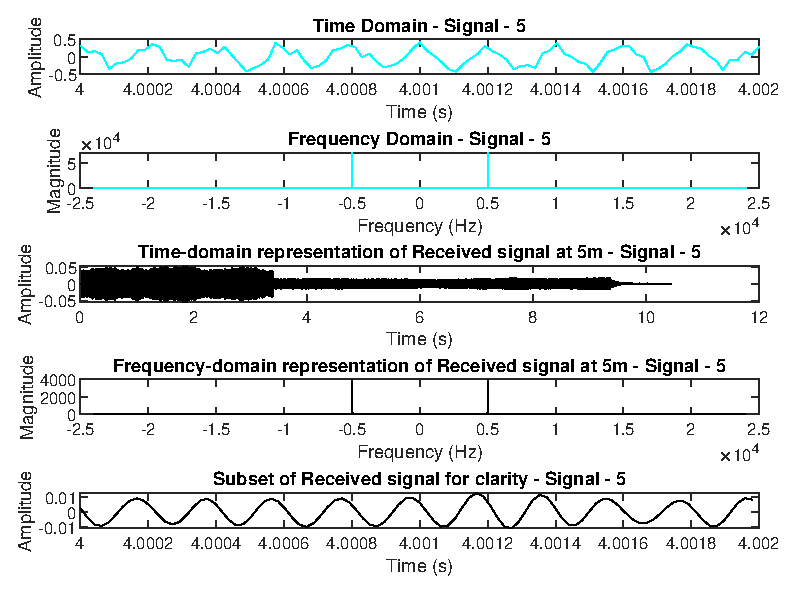
\includegraphics[width=1.1\linewidth]{5_5.eps}


\newpage
\section{Impact of Distance of Separation on Frequency Profile }
The influence of distance separation, varying from 1 to 5 meters, on both frequency and time domain signals is observed to be simultaneously  profound and subtle. First glance at the graphs makes it clear that with increasing distance the amplitude of the received waveform is decreasing. In the frequency domain, the attenuation of signals becomes more pronounced with increasing distance, resulting in a decrease in signal strength. Moreover, as the distance increases, the propagation delay becomes more significant, leading to temporal spreading of the signal in the time domain. This temporal spreading manifests as a widening of the signal's pulse duration, ultimately affecting the fidelity and reliability of communication systems, particularly in scenarios where precise timing is crucial. The propagation delay also results in phase shifts that we can see from the graphs.   





\section{Deciphering Discrepancies: Investigating variances in triangle signal transmission}
When transmitting a triangle signal and examining its frequency domain representation, we typically encounter a  $ \sinc^2(f) $ 
graph, which is theoretically band-unlimited. However, upon reception, the signal often appears as a smoother version of the transmitted triangle. This discrepancy arises not from the selective loss of frequencies during transmission but rather due to the effects of attenuation, distortion, and noise inherent in the transmission channel. These factors collectively contribute to altering the frequency components and overall shape of the received signal. Consequently, the received signal appears smoother than the original triangle, reflecting the cumulative impact of these transmission channel characteristics.

\section{Revealing the Rhythm: How Noise Cancellation Creates Periodic Signals}
When a sinusoidal signal contaminated with noise was transmitted and subsequently captured using a microphone (which is capable of accurately recording frequencies up to 22kHz), upon examination, the received signal displayed a waveform closely resembling a sinusoid, suggesting successful transmission and reception. Notably, the microphone effectively suppressed the noise, leading to a clearer representation of the transmitted signal.


\section{Microphone Specification}

\begin{figure}[h]
    \centering
    \includegraphics[width=1\linewidth]{mic_spec.png}
    \caption{Specs}
    \label{fig:enter-label}
\end{figure}






\section{Audio Signal Generation}

\begin{lstlisting}

fs = 48000;
duration = 10;
t = linspace(0,duration,fs*duration);

% Recording__1
y1 = 1*cos(2*pi*5000*t);
audiowrite('./audio1.wav',y1,fs);

% Recording__2
y2 = 0.9*sin(2*pi*10000*t);

audiowrite('./audio2.wav',y2,fs);

% Recording__3 
y3 = 0.5*sin(2*pi*10000*t)+0.3*cos(2*pi*10000*t);
audiowrite('./audio3.wav',y3,fs);

% Recording__4
y4 = 0.8*triangle(2 * pi * 2000 * t, 0.5);
audiowrite('./audio4.wav',y4,fs);

% Recording__5
noise = 0.1 * randn(size(t));
y5 = 0.3*cos(2*pi*5000*t) + noise;
audiowrite('./audio5.wav',y5,fs);

\end{lstlisting}



\section{Tuning for the selected Duration}


\begin{lstlisting}
% Time domain signals figure
% Define the time interval for clearer visualization
start_time = 0.1; % Start time in seconds
end_time = 0.11;   % End time in seconds
duration = end_time - start_time; % Duration in seconds

% Generate time vector for the specified interval
t_interval = linspace(start_time, end_time, fs * duration);

% Generate signals using the specified time interval
y1_interval = 1*cos(2*pi*5000*t_interval);
y2_interval = 0.9*sin(2*pi*1000*t_interval);
y3_interval = 0.5*sin(2*pi*3000*t_interval)+0.3*cos(2*pi*6000*t_interval);
y4_interval = 0.8*triangle(2 * pi * 2000 * t_interval, 0.5);
noise_interval = 0.1 * randn(size(t_interval));
y5_interval = 0.3*cos(2*pi*5000*t_interval) + noise_interval;
\end{lstlisting}



\section{Audio Signal Capture}

\begin{lstlisting}
% Load the WAV file
[y, fs] = audioread('./audio2_500Hz.wav');


% Calculate the time axis
num_samples = length(y);
time_axis = (0:num_samples-1) / fs;

Y = fftshift(fft(y));
f_axis = -fs/2:fs/(length(Y)-1):fs/2;
f_axis = f_axis';


% Plot the frequency-domain representation
figure;
subplot(2,1,1);
plot(f_axis, abs(Y));
xlabel('Frequency (Hz)');
ylabel('Magnitude');



% Plot the time-domain representation
subplot(2,1,2);
plot(time_axis, y);
xlabel('Time (seconds)');
ylabel('Amplitude');
title('Time-domain representation of example.wav');
\end{lstlisting}



\section{Automation in MATLAB - Efficient way to get all done}

\begin{lstlisting}

clc;
clear;
close all;

% 3 automation magic :-

% 1
signals = {@(t) 1*cos(2*pi*5000*t), ...
           @(t) 0.9*sin(2*pi*1000*t), ...
           @(t) 0.5*sin(2*pi*3000*t)+0.3*cos(2*pi*6000*t), ...
           @(t) 0.8*triangle(2 * pi * 2000 * t, 0.5), ...
           @(t) 0.3*cos(2*pi*5000*t) + 0.1 * randn(size(t))};


% 2
colors = {'r', 'g', 'b', 'm', 'c'};



% 3
received_files = {'./DSP_PROJECT__1/3_r1.wav', ...
                  './DSP_PROJECT__1/3_r2.wav', ...
                  './DSP_PROJECT__1/3_r3.wav', ...
                  './DSP_PROJECT__1/3_r4.wav', ...
                  './DSP_PROJECT__1/3_r5.wav'};





for i = 1:numel(signals)
    
    fs_generated = 48000;
    duration_ = 10;
    t = linspace(0,duration_ ,fs_generated * duration_);
    y1 = signals{i}(t);
    
    
    % Time interval for clearer Visualization
    start_time = 4;  
    end_time = 4.002;
    duration = end_time - start_time; 

    % Generating time vector for THAT specified interval
    t1_interval = linspace(start_time, end_time, fs_generated * duration);
    y1_interval = signals{i}(t1_interval);




    % Define subplot title according to signal
    subplot_title = sprintf('Signal - %d', i);
    



    % Plot time-domain representation of TRANSMITTED SIGNAL
    figure;
    subplot(5, 1, 1);
    plot(t1_interval, y1_interval, colors{i});
    title(['Time Domain - ' subplot_title]);
    xlabel('Time (s)');
    ylabel('Amplitude');
    

    % Plot frequency-domain representation of TRANSMITTED SIGNAL
    subplot(5, 1, 2);

    Y1 = fftshift(fft(y1));
    frequencies = linspace(-fs_generated/2, fs_generated/2, length(Y1));
    
    plot(frequencies, abs(Y1), colors{i});
    title(['Frequency Domain - ' subplot_title]);
    xlabel('Frequency (Hz)');
    ylabel('Magnitude');
    








    % Read received signal and extract subset
    [y_received, fs_received] = audioread(received_files{i});
    num_samples = length(y_received);
    time_axis_received = (0:num_samples-1) / fs_received;
  
    % Plot time domain of RECEIVED SIGNAL
    subplot(5, 1, 3);
    plot(time_axis_received, y_received, 'k');
    xlabel('Time (s)');
    ylabel('Amplitude');
    title(['Time-domain representation of Received signal at 3m - ...
    ' subplot_title]);


    Y_received = fftshift(fft(y_received));
    f_axis_received = -fs_received/2 : fs_received/(length(Y_received)-1) ...
    : fs_received/2;
    f_axis_received = f_axis_received';

    subplot(5, 1, 4);
    plot(f_axis_received, abs(Y_received), 'k');
    xlabel('Frequency (Hz)');
    ylabel('Magnitude');
    title(['Frequency-domain representation of Received signal at 3m - ...
    ' subplot_title]);











    % Indexes corresponding to start and end time
    start_index = round(start_time * fs_received ) + 1;
    end_index = round(end_time * fs_received );

    % Extract samples from the specified time range
    y_subset = y_received(start_index:end_index);
    time_subset = time_axis_received(start_index:end_index);   

    subplot(5, 1, 5);
    plot(time_subset, y_subset, 'k');
    xlabel('Time (s)');
    ylabel('Amplitude');
    title(['Subset of Received signal for clarity - ' subplot_title]);
    

    % Save figure as EPS file
    print(gcf, '-depsc', sprintf('1_%d.eps', i));

end

\end{lstlisting}



\chapter{ Frequency Specification of Microphone }

\section{Introduction}

We searched for the data sheet for the Microphone we were using. Parameters we were focused on are :-
\begin{itemize}
    \item Range of Frequencies we can operate in
    \item Transfer Characteristics
    \item Filter Algorithms used for Noise cancellation
\end{itemize}

Since these specifications were not available, possible because of proprietary reasons, we decided to probe at least the range of frequencies that we can operate in, on our own. We decided to send a simple sine wave of different frequencies ranging from very small ($\approx 100$ Hz) to pretty high ( $\approx  23k$ Hz ) values. The idea is to check for which range of values we get the signal frequencies and waveform accurate and where do the cut off points lie. 






\section{Cut Off Frequency Probing}



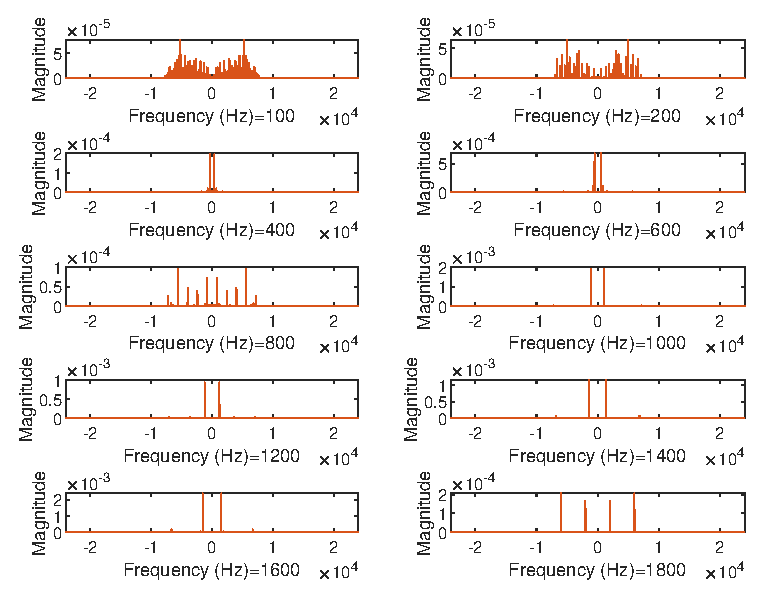
\includegraphics[width=1\linewidth]{first_10.eps}

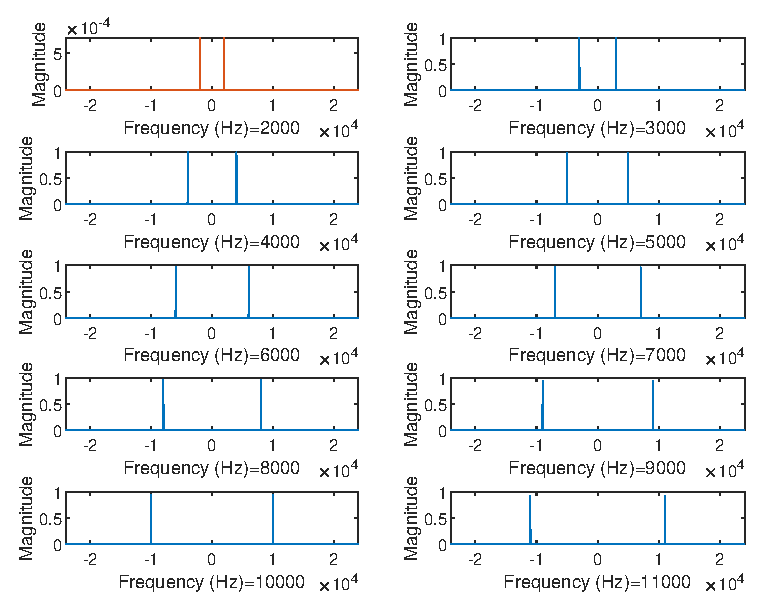
\includegraphics[width=1\linewidth]{next_10.eps}

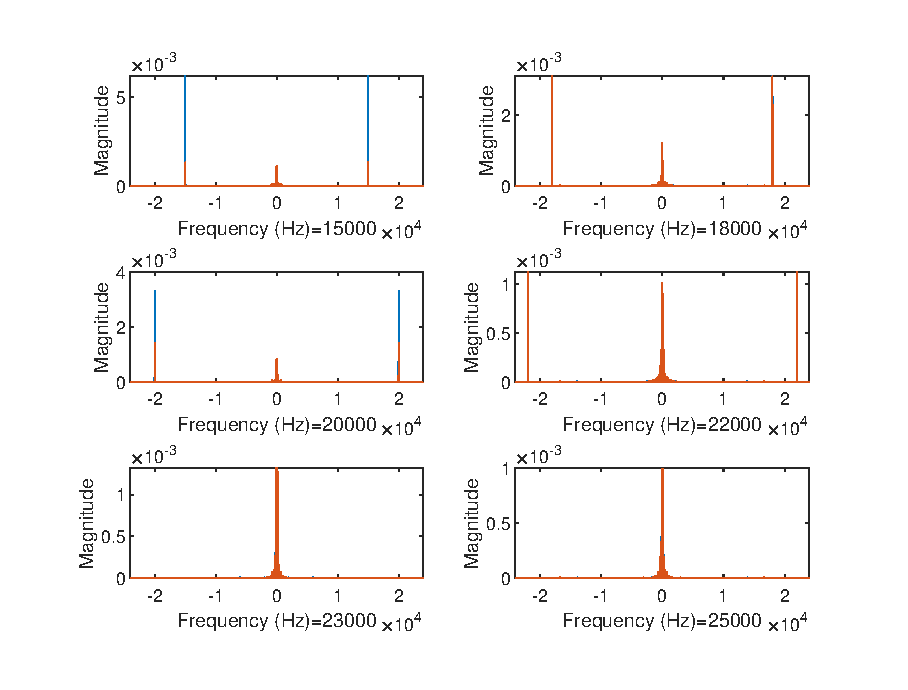
\includegraphics[width=1\linewidth]{last_six.eps}


\newpage

\section{Limits Observed}

\begin{figure}[H]
    \centering
    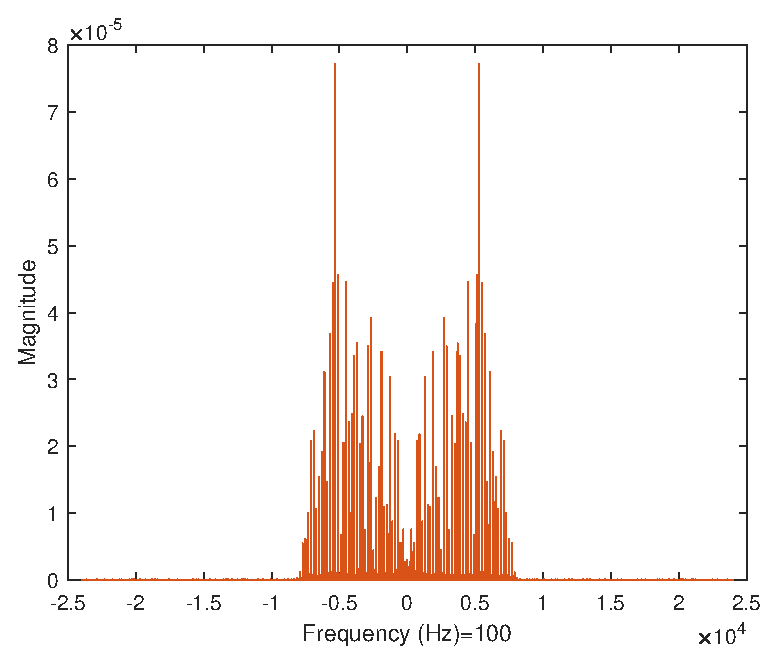
\includegraphics[width=0.7\linewidth]{small_anamoly.eps}
    \caption{100 Hz received profile}
    \label{fig:enter-label}
\end{figure}


\begin{figure}[H]
    \centering
    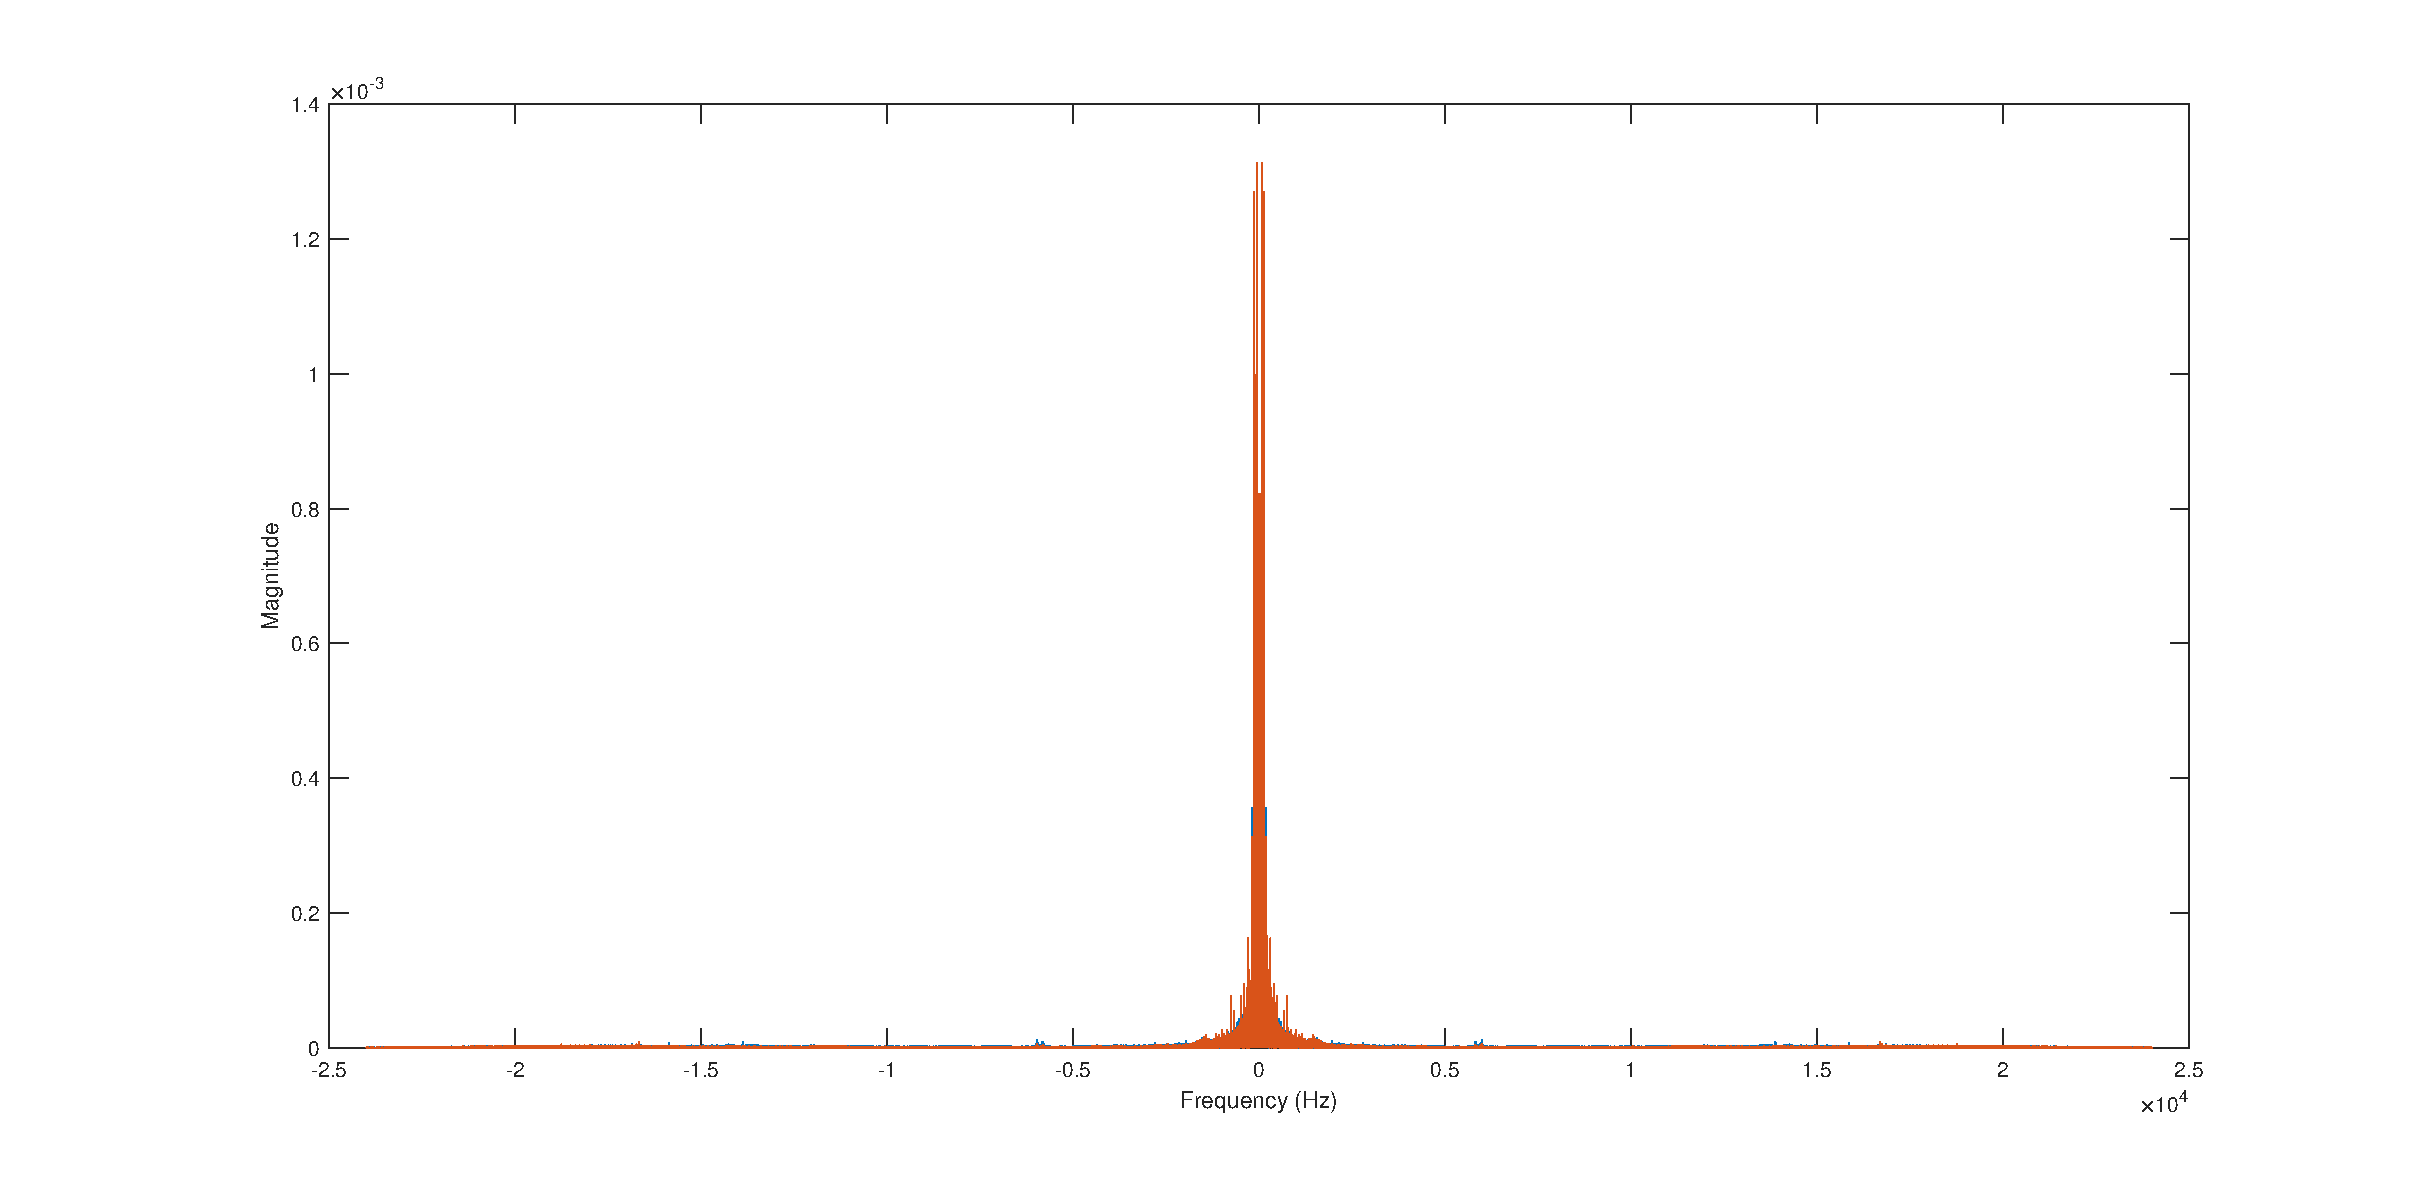
\includegraphics[width=1\linewidth]{23k.eps}
    \caption{23,000 Hz received profile}
    \label{fig:enter-label}
\end{figure}

\newpage


\section{Proof of Concept for Better Probing}


\begin{itemize}
    \item \textbf{Transmitting a $\sinc$ Signal } :- Instead of checking for individual frequencies, it would be faster to choose a $\rect$ that encompasses a range of frequencies we want to probe. Say a $\rect \left( \frac{f}{15k} \right) $  is the range of frequencies we want to probe on, then we send a signal of $\frac{1}{15k}\sinc_{\pi}\left( t \cdot 15k \right)$ which isn't technically feasible since the audio file generated proved to be too long even after windowing out in time domain. Transmitting almost 10 minutes of audio in a noiseless environment proved to be challenging.  
    
    \item \textbf{Binary Searching the Cut off Frequencies :- } This is probably the most efficient way since we have an approximate idea that the microphones should probably operate close to human's audible range, so we could have chose low as 15k and high as 25k. Then we could increase upper bound until we reach a point where the microphone gives wrong answer. Then binary search between high and low. Applicable for finding both upper and lower bounds.

\begin{lstlisting}
low = high = 15k

if Recieved high is correct :
	low = high
	high += 5k

// Binary search between high and low 
// to find precisely where is cut off frequency
// for upper bound is

\end{lstlisting}

We do the same to find lower bound also.

\begin{lstlisting}
low = high = 5k

if Recieved low is correct :
	high = low
	low -= 1k

// Binary search between high and low 
// to find precisely where is cut off frequency
// for lower bound is
\end{lstlisting}

\end{itemize}


\section{References}

\begin{itemize}
    \item \url{https://in.mathworks.com/help/matlab/ref/sound.html}
    \item  \url{https://in.mathworks.com/help/matlab/ref/fft.html}
\end{itemize}



\end{document}